\documentclass[a4paper,landscape]{article}
\usepackage[margin=0.5cm]{geometry}
\usepackage{tikz}
\usepackage[T1]{fontenc}
\usepackage{lmodern}
\usepackage{amssymb}
\usepackage{xcolor}
\usetikzlibrary{arrows.meta,positioning,fit,backgrounds,calc}

\definecolor{Ci}{RGB}{52,152,219}
\definecolor{Cq}{RGB}{155,89,182}
\definecolor{Cl}{RGB}{243,156,18}
\definecolor{Cs}{RGB}{39,174,96}
\definecolor{Cd}{RGB}{230,126,34}
\definecolor{Cv}{RGB}{231,76,60}
\definecolor{Cf}{RGB}{22,160,133}
\definecolor{Cp}{RGB}{44,62,80}
\definecolor{Cw}{RGB}{100,120,130}
\definecolor{Cr}{RGB}{192,57,43}
\definecolor{Co}{RGB}{52,73,94}

\tikzset{
  SH/.style={rectangle,rounded corners=3pt,
    draw=#1!85!black,fill=#1!72,text=white,
    font=\bfseries\scriptsize,inner sep=4pt,align=center},
  CB/.style={rectangle,rounded corners=2pt,
    draw=#1!60!black,fill=#1!11,
    font=\scriptsize,inner sep=3pt,align=center},
  IP/.style={rectangle,rounded corners=2pt,
    draw=#1!45!black,fill=#1!7,
    font=\tiny,inner sep=3pt,align=left},
  RG/.style={rectangle,rounded corners=6pt,
    draw=#1!38!black,fill=#1!4,
    dashed,inner sep=6pt},
  fw/.style={-{Stealth[length=4pt,width=3pt]},thick,#1},
  bk/.style={-{Stealth[length=4pt,width=3pt]},thick,Cl!80!black,
    rounded corners=4pt},
  rj/.style={-{Stealth[length=4pt,width=3pt]},thick,Cr,dashed}
}

%% All column headers placed at the same y=−1.3cm (absolute coords).
%% x positions chosen so fit nodes do not overlap.
%%   Col  tw   xhdr
%%    1  3.1    0.0
%%    2  3.0    4.1
%%    3  2.3    7.9
%%    4  4.1   11.0
%%    5  3.1   15.9
%%    6  3.7   19.8
%%    7  3.2   24.2

\begin{document}
\pagestyle{empty}
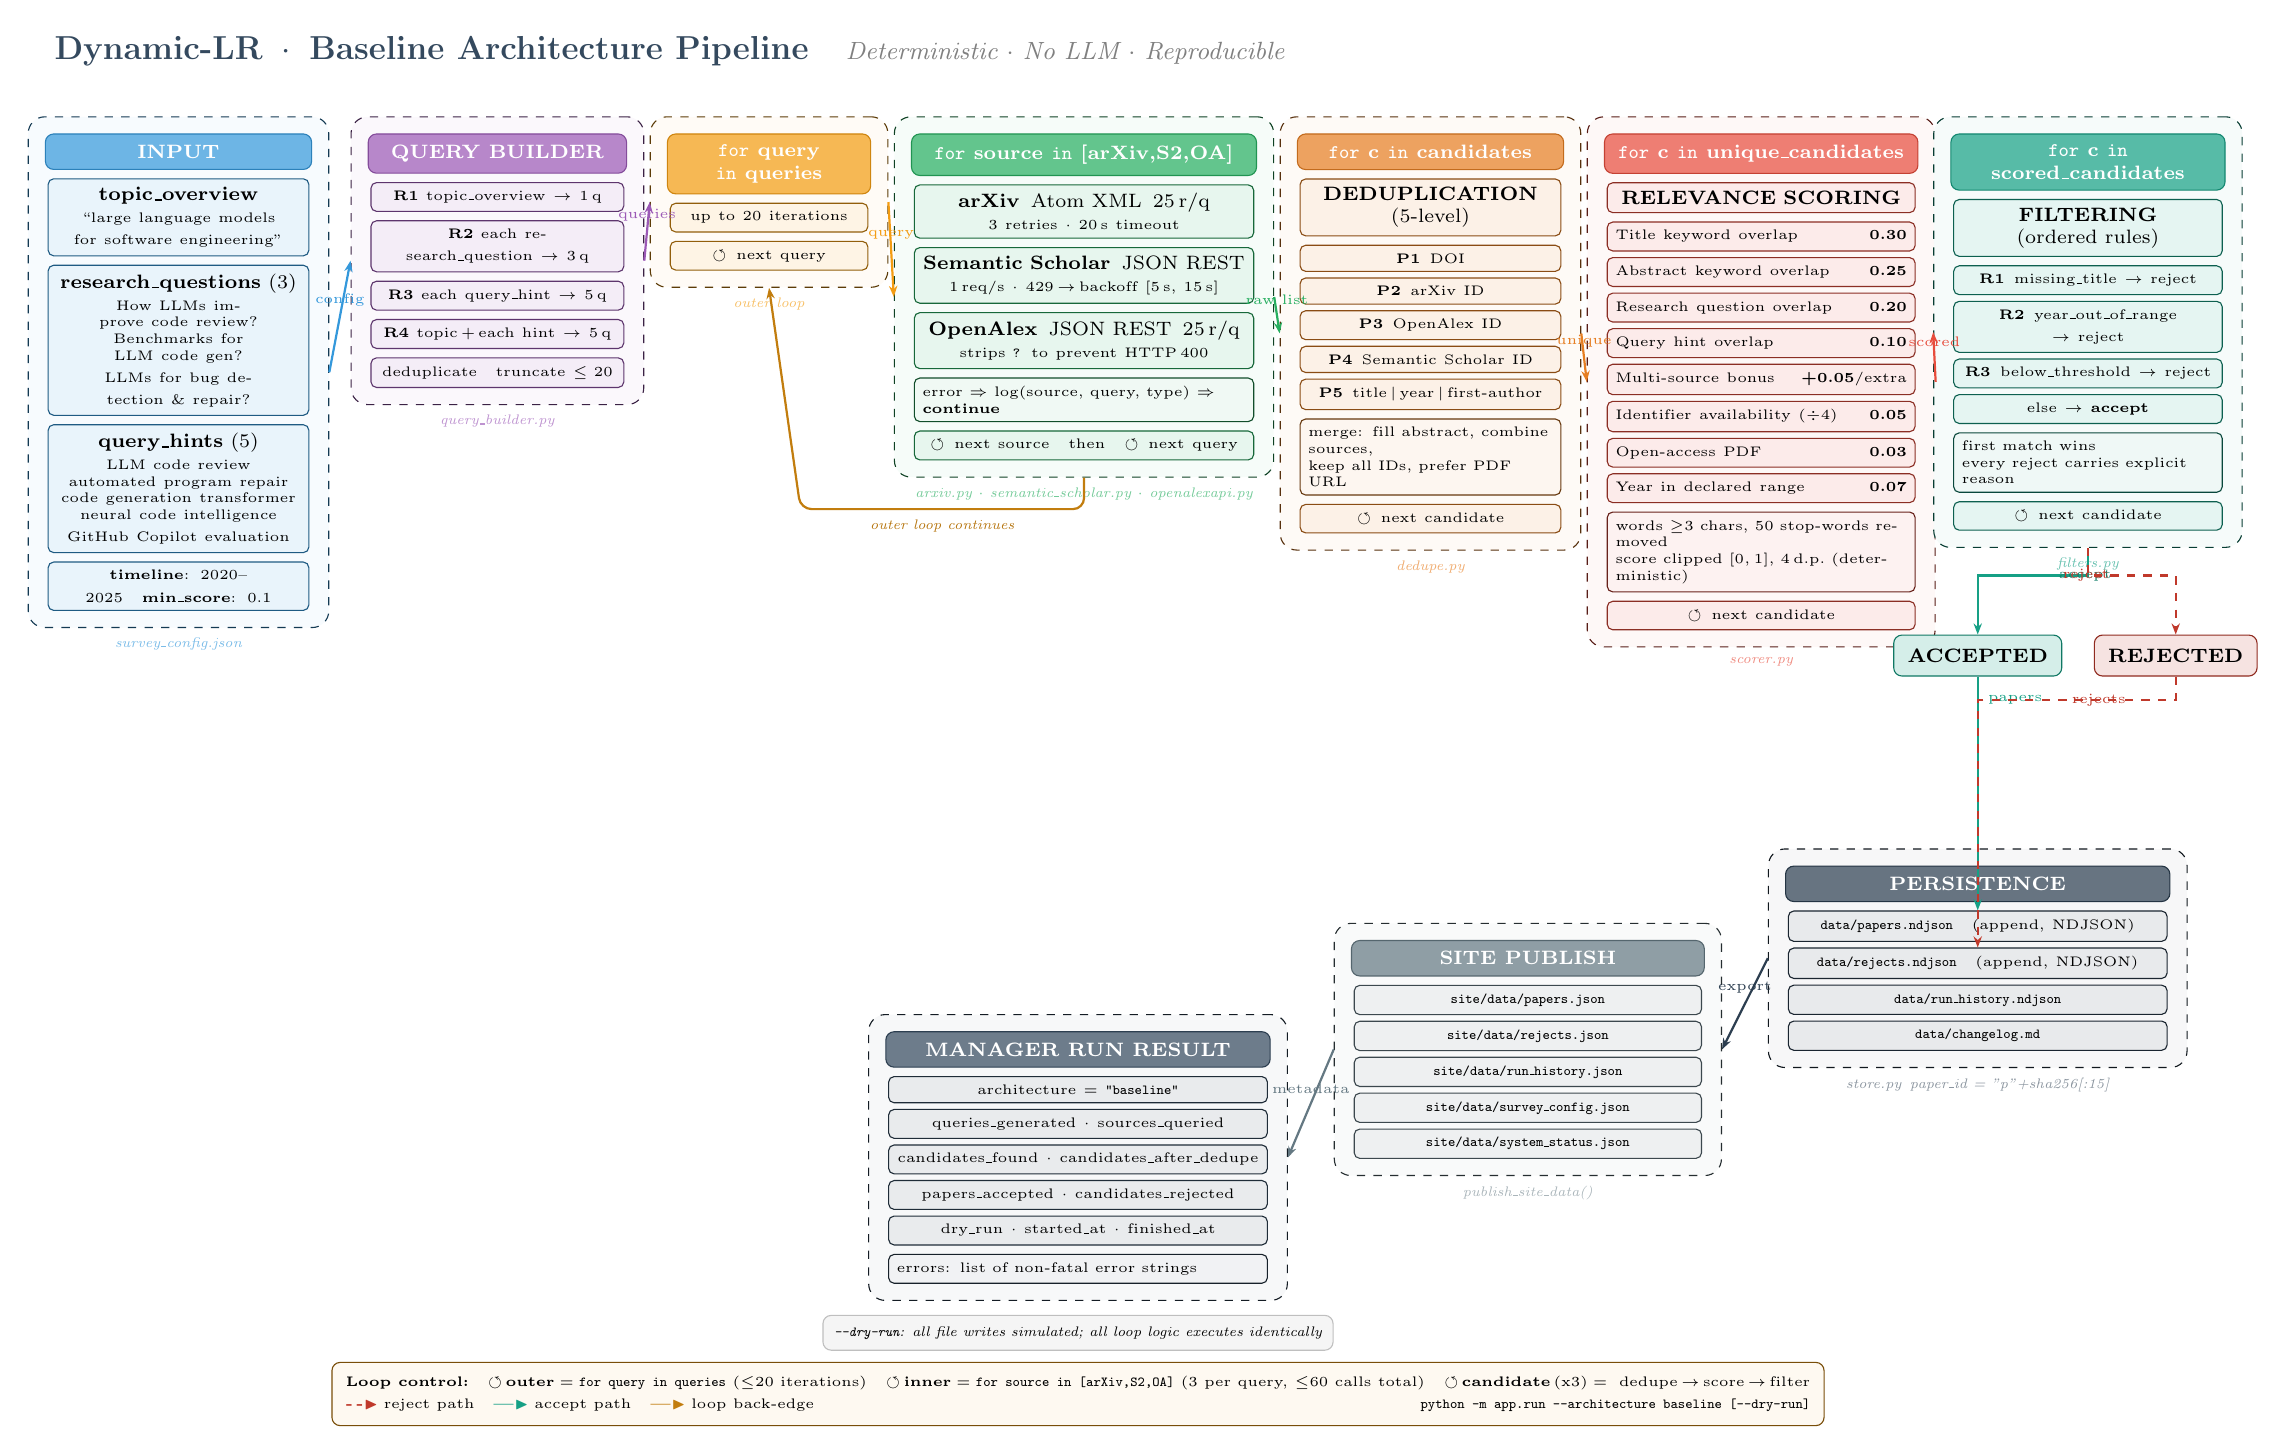
\begin{tikzpicture}[node distance=3pt]

%% ── TITLE ──────────────────────────────────────────────────────────────────
\node[font=\large\bfseries,text=Co,anchor=north west] (TTL)
  at (0,0)
  {Dynamic-LR\enspace$\cdot$\enspace Baseline Architecture Pipeline\quad
   {\normalfont\small\itshape\textcolor{gray}{Deterministic $\cdot$ No LLM $\cdot$ Reproducible}}};

%% ── y anchor shared by all stage headers ───────────────────────────────────
\coordinate (Y0) at (0,-1.35cm);

%% ══════════════════════════════════════════════════════════════════════
%%  COL 1 — INPUT   (xhdr=0)
%% ══════════════════════════════════════════════════════════════════════
\node[SH=Ci,text width=3.1cm,anchor=north west] (H1) at (0,-1.35cm) {INPUT};

\node[CB=Ci,text width=3.1cm,below=3pt of H1] (C1a)
  {\textbf{topic\_overview}\\[2pt]
   \tiny ``large language models\\for software engineering''};

\node[CB=Ci,text width=3.1cm,below=3pt of C1a] (C1b)
  {\textbf{research\_questions}~(3)\\[2pt]
   \tiny How LLMs improve code review?\\
   Benchmarks for LLM code gen?\\
   LLMs for bug detection \& repair?};

\node[CB=Ci,text width=3.1cm,below=3pt of C1b] (C1c)
  {\textbf{query\_hints}~(5)\\[2pt]
   \tiny LLM code review\\
   automated program repair\\
   code generation transformer\\
   neural code intelligence\\
   GitHub Copilot evaluation};

\node[CB=Ci,text width=3.1cm,below=3pt of C1c] (C1d)
  {\tiny\textbf{timeline}: 2020--2025\quad\textbf{min\_score}: 0.1};

\begin{scope}[on background layer]
\node[RG=Ci,fit=(H1)(C1a)(C1b)(C1c)(C1d),
      label={[font=\tiny\itshape,Ci!65]below:survey\_config.json}] (R1) {};
\end{scope}

%% ══════════════════════════════════════════════════════════════════════
%%  COL 2 — QUERY BUILDER   (xhdr=4.1)
%% ══════════════════════════════════════════════════════════════════════
\node[SH=Cq,text width=3.0cm,anchor=north west] (H2) at (4.1cm,-1.35cm)
  {QUERY BUILDER};

\node[CB=Cq,text width=3.0cm,below=3pt of H2] (C2a)
  {\tiny\textbf{R1} topic\_overview $\to$ 1\,q};
\node[CB=Cq,text width=3.0cm,below=3pt of C2a] (C2b)
  {\tiny\textbf{R2} each research\_question $\to$ 3\,q};
\node[CB=Cq,text width=3.0cm,below=3pt of C2b] (C2c)
  {\tiny\textbf{R3} each query\_hint $\to$ 5\,q};
\node[CB=Cq,text width=3.0cm,below=3pt of C2c] (C2d)
  {\tiny\textbf{R4} topic\,+\,each hint $\to$ 5\,q};
\node[CB=Cq,text width=3.0cm,below=3pt of C2d] (C2e)
  {\tiny deduplicate\quad truncate $\leq 20$};

\begin{scope}[on background layer]
\node[RG=Cq,fit=(H2)(C2a)(C2b)(C2c)(C2d)(C2e),
      label={[font=\tiny\itshape,Cq!65]below:query\_builder.py}] (R2) {};
\end{scope}

%% ══════════════════════════════════════════════════════════════════════
%%  COL 3 — OUTER LOOP   (xhdr=7.9)
%% ══════════════════════════════════════════════════════════════════════
\node[SH=Cl,text width=2.3cm,anchor=north west] (H3) at (7.9cm,-1.35cm)
  {\texttt{for} query\\\texttt{in} queries};

\node[CB=Cl,text width=2.3cm,below=3pt of H3] (C3a)
  {\tiny up to 20 iterations};
\node[CB=Cl,text width=2.3cm,below=3pt of C3a] (C3b)
  {\tiny$\circlearrowleft$\enspace next query};

\begin{scope}[on background layer]
\node[RG=Cl,fit=(H3)(C3a)(C3b),
      label={[font=\tiny\itshape,Cl!65]below:outer loop}] (R3) {};
\end{scope}

%% ══════════════════════════════════════════════════════════════════════
%%  COL 4 — INNER LOOP / SOURCE SEARCH   (xhdr=11.0)
%% ══════════════════════════════════════════════════════════════════════
\node[SH=Cs,text width=4.1cm,anchor=north west] (H4) at (11.0cm,-1.35cm)
  {\texttt{for} source \texttt{in} [arXiv,S2,OA]};

\node[CB=Cs,text width=4.1cm,below=3pt of H4] (C4a)
  {\textbf{arXiv}\enspace Atom XML\enspace 25\,r/q\\
   \tiny 3 retries $\cdot$ 20\,s timeout};
\node[CB=Cs,text width=4.1cm,below=3pt of C4a] (C4b)
  {\textbf{Semantic Scholar}\enspace JSON REST\\
   \tiny 1\,req/s $\cdot$ 429\,$\to$\,backoff [5\,s, 15\,s]};
\node[CB=Cs,text width=4.1cm,below=3pt of C4b] (C4c)
  {\textbf{OpenAlex}\enspace JSON REST\enspace 25\,r/q\\
   \tiny strips \texttt{?} to prevent HTTP\,400};
\node[IP=Cs,text width=4.1cm,below=3pt of C4c] (C4d)
  {error $\Rightarrow$ log(source, query, type) $\Rightarrow$ \textbf{continue}};
\node[CB=Cs,text width=4.1cm,below=3pt of C4d] (C4e)
  {\tiny$\circlearrowleft$\enspace next source\quad then\quad$\circlearrowleft$\enspace next query};

\begin{scope}[on background layer]
\node[RG=Cs,fit=(H4)(C4a)(C4b)(C4c)(C4d)(C4e),
      label={[font=\tiny\itshape,Cs!65]below:arxiv.py $\cdot$ semantic\_scholar.py $\cdot$ openalexapi.py}]
      (R4) {};
\end{scope}

%% outer-loop back-edge arrow
\draw[bk] (R4.south) -- ++(0,-0.4)
  -- node[below,font=\tiny\itshape,text=Cl!75!black]{outer loop continues}
  ++(-3.6cm,0) -- (R3.south);

%% ══════════════════════════════════════════════════════════════════════
%%  COL 5 — DEDUPLICATION   (xhdr=15.9)
%% ══════════════════════════════════════════════════════════════════════
\node[SH=Cd,text width=3.1cm,anchor=north west] (H5) at (15.9cm,-1.35cm)
  {\texttt{for} c \texttt{in} candidates};

\node[CB=Cd,text width=3.1cm,below=3pt of H5] (C5t)
  {\scriptsize\textbf{DEDUPLICATION} (5-level)};
\node[CB=Cd,text width=3.1cm,below=3pt of C5t] (C5a)
  {\tiny\textbf{P1}\enspace DOI};
\node[CB=Cd,text width=3.1cm,below=2pt of C5a] (C5b)
  {\tiny\textbf{P2}\enspace arXiv ID};
\node[CB=Cd,text width=3.1cm,below=2pt of C5b] (C5c)
  {\tiny\textbf{P3}\enspace OpenAlex ID};
\node[CB=Cd,text width=3.1cm,below=2pt of C5c] (C5d)
  {\tiny\textbf{P4}\enspace Semantic Scholar ID};
\node[CB=Cd,text width=3.1cm,below=2pt of C5d] (C5e)
  {\tiny\textbf{P5}\enspace title\,$|$\,year\,$|$\,first-author};
\node[IP=Cd,text width=3.1cm,below=3pt of C5e] (C5f)
  {merge: fill abstract, combine sources,\\keep all IDs, prefer PDF URL};
\node[CB=Cd,text width=3.1cm,below=3pt of C5f] (C5g)
  {\tiny$\circlearrowleft$\enspace next candidate};

\begin{scope}[on background layer]
\node[RG=Cd,fit=(H5)(C5t)(C5a)(C5b)(C5c)(C5d)(C5e)(C5f)(C5g),
      label={[font=\tiny\itshape,Cd!65]below:dedupe.py}] (R5) {};
\end{scope}

%% ══════════════════════════════════════════════════════════════════════
%%  COL 6 — RELEVANCE SCORING   (xhdr=19.8)
%% ══════════════════════════════════════════════════════════════════════
\node[SH=Cv,text width=3.7cm,anchor=north west] (H6) at (19.8cm,-1.35cm)
  {\texttt{for} c \texttt{in} unique\_candidates};

\node[CB=Cv,text width=3.7cm,below=3pt of H6] (C6t)
  {\scriptsize\textbf{RELEVANCE SCORING}};
\node[CB=Cv,text width=3.7cm,below=3pt of C6t] (C6a)
  {\tiny Title keyword overlap\hspace{\fill}\textbf{0.30}};
\node[CB=Cv,text width=3.7cm,below=2pt of C6a] (C6b)
  {\tiny Abstract keyword overlap\hspace{\fill}\textbf{0.25}};
\node[CB=Cv,text width=3.7cm,below=2pt of C6b] (C6c)
  {\tiny Research question overlap\hspace{\fill}\textbf{0.20}};
\node[CB=Cv,text width=3.7cm,below=2pt of C6c] (C6d)
  {\tiny Query hint overlap\hspace{\fill}\textbf{0.10}};
\node[CB=Cv,text width=3.7cm,below=2pt of C6d] (C6e)
  {\tiny Multi-source bonus\hspace{\fill}\textbf{+0.05}/extra};
\node[CB=Cv,text width=3.7cm,below=2pt of C6e] (C6f)
  {\tiny Identifier availability ($\div$4)\hspace{\fill}\textbf{0.05}};
\node[CB=Cv,text width=3.7cm,below=2pt of C6f] (C6g)
  {\tiny Open-access PDF\hspace{\fill}\textbf{0.03}};
\node[CB=Cv,text width=3.7cm,below=2pt of C6g] (C6h)
  {\tiny Year in declared range\hspace{\fill}\textbf{0.07}};
\node[IP=Cv,text width=3.7cm,below=3pt of C6h] (C6i)
  {words $\geq$3 chars, 50 stop-words removed\\
   score clipped $[0,1]$, 4\,d.p.~(deterministic)};
\node[CB=Cv,text width=3.7cm,below=3pt of C6i] (C6j)
  {\tiny$\circlearrowleft$\enspace next candidate};

\begin{scope}[on background layer]
\node[RG=Cv,fit=(H6)(C6t)(C6a)(C6b)(C6c)(C6d)(C6e)(C6f)(C6g)(C6h)(C6i)(C6j),
      label={[font=\tiny\itshape,Cv!65]below:scorer.py}] (R6) {};
\end{scope}

%% ══════════════════════════════════════════════════════════════════════
%%  COL 7 — FILTERING   (xhdr=24.2)
%% ══════════════════════════════════════════════════════════════════════
\node[SH=Cf,text width=3.2cm,anchor=north west] (H7) at (24.2cm,-1.35cm)
  {\texttt{for} c \texttt{in} scored\_candidates};

\node[CB=Cf,text width=3.2cm,below=3pt of H7] (C7t)
  {\scriptsize\textbf{FILTERING} (ordered rules)};
\node[CB=Cf,text width=3.2cm,below=3pt of C7t] (C7a)
  {\tiny\textbf{R1}\enspace missing\_title $\to$ reject};
\node[CB=Cf,text width=3.2cm,below=2pt of C7a] (C7b)
  {\tiny\textbf{R2}\enspace year\_out\_of\_range $\to$ reject};
\node[CB=Cf,text width=3.2cm,below=2pt of C7b] (C7c)
  {\tiny\textbf{R3}\enspace below\_threshold $\to$ reject};
\node[CB=Cf,text width=3.2cm,below=2pt of C7c] (C7d)
  {\tiny else $\to$ \textbf{accept}};
\node[IP=Cf,text width=3.2cm,below=3pt of C7d] (C7e)
  {first match wins\\every reject carries explicit reason};
\node[CB=Cf,text width=3.2cm,below=3pt of C7e] (C7f)
  {\tiny$\circlearrowleft$\enspace next candidate};

\begin{scope}[on background layer]
\node[RG=Cf,fit=(H7)(C7t)(C7a)(C7b)(C7c)(C7d)(C7e)(C7f),
      label={[font=\tiny\itshape,Cf!65]below:filters.py}] (R7) {};
\end{scope}

%% ══════════════════════════════════════════════════════════════════════
%%  ACCEPT / REJECT SPLIT
%% ══════════════════════════════════════════════════════════════════════
\node[rectangle,rounded corners=3pt,
      draw=Cf!75!black,fill=Cf!18,font=\scriptsize\bfseries,inner sep=5pt,
      below=1.1cm of R7.south,xshift=-1.4cm] (ACC) {ACCEPTED};

\node[rectangle,rounded corners=3pt,
      draw=Cr!75!black,fill=Cr!14,font=\scriptsize\bfseries,inner sep=5pt,
      right=0.4cm of ACC] (REJ) {REJECTED};

\draw[fw=Cf] (R7.south) -- ++(0,-0.35) -| (ACC.north)
  node[pos=0.18,right,font=\tiny,Cf!80!black]{accept};
\draw[rj]    (R7.south) -- ++(0,-0.35) -| (REJ.north)
  node[pos=0.18,left,font=\tiny,Cr]{reject};

%% ══════════════════════════════════════════════════════════════════════
%%  BOTTOM ROW — positioned relative to ACCEPT/REJECT nodes
%% ══════════════════════════════════════════════════════════════════════

%%  PERSISTENCE
\node[SH=Cp,text width=4.6cm,
      below=2.4cm of ACC.south,anchor=north] (HP) {PERSISTENCE};

\node[CB=Cp,text width=4.6cm,below=3pt of HP] (Pa)
  {\tiny\texttt{data/papers.ndjson}\quad(append, NDJSON)};
\node[CB=Cp,text width=4.6cm,below=2pt of Pa] (Pb)
  {\tiny\texttt{data/rejects.ndjson}\quad(append, NDJSON)};
\node[CB=Cp,text width=4.6cm,below=2pt of Pb] (Pc)
  {\tiny\texttt{data/run\_history.ndjson}};
\node[CB=Cp,text width=4.6cm,below=2pt of Pc] (Pd)
  {\tiny\texttt{data/changelog.md}};

\begin{scope}[on background layer]
\node[RG=Cp,fit=(HP)(Pa)(Pb)(Pc)(Pd),
      label={[font=\tiny\itshape,Cp!55]below:store.py\enspace paper\_id = "p"+sha256[:15]}]
      (RP) {};
\end{scope}

\draw[fw=Cf] (ACC.south) -- ++(0,-0.3) -| (Pa.north)
  node[pos=0.1,right,font=\tiny]{papers};
\draw[rj]    (REJ.south) -- ++(0,-0.3) -| (Pb.north)
  node[pos=0.1,left,font=\tiny]{rejects};

%%  SITE PUBLISH
\node[SH=Cw,text width=4.2cm,
      left=0.8cm of RP.west,anchor=east] (HW) {SITE PUBLISH};

\node[CB=Cw,text width=4.2cm,below=3pt of HW] (Wa)
  {\tiny\texttt{site/data/papers.json}};
\node[CB=Cw,text width=4.2cm,below=2pt of Wa] (Wb)
  {\tiny\texttt{site/data/rejects.json}};
\node[CB=Cw,text width=4.2cm,below=2pt of Wb] (Wc)
  {\tiny\texttt{site/data/run\_history.json}};
\node[CB=Cw,text width=4.2cm,below=2pt of Wc] (Wd)
  {\tiny\texttt{site/data/survey\_config.json}};
\node[CB=Cw,text width=4.2cm,below=2pt of Wd] (We)
  {\tiny\texttt{site/data/system\_status.json}};

\begin{scope}[on background layer]
\node[RG=Cw,fit=(HW)(Wa)(Wb)(Wc)(Wd)(We),
      label={[font=\tiny\itshape,Cw!55]below:publish\_site\_data()}]
      (RW) {};
\end{scope}

\draw[fw=Cp] (RP.west) -- node[above,font=\tiny]{export} (RW.east);

%%  MANAGER RUN RESULT
\node[SH=Co,text width=4.6cm,
      left=0.8cm of RW.west,anchor=east] (HO) {MANAGER RUN RESULT};

\node[CB=Co,text width=4.6cm,below=3pt of HO] (Oa)
  {\tiny architecture = \texttt{"baseline"}};
\node[CB=Co,text width=4.6cm,below=2pt of Oa] (Ob)
  {\tiny queries\_generated $\cdot$ sources\_queried};
\node[CB=Co,text width=4.6cm,below=2pt of Ob] (Oc)
  {\tiny candidates\_found $\cdot$ candidates\_after\_dedupe};
\node[CB=Co,text width=4.6cm,below=2pt of Oc] (Od)
  {\tiny papers\_accepted $\cdot$ candidates\_rejected};
\node[CB=Co,text width=4.6cm,below=2pt of Od] (Oe)
  {\tiny dry\_run $\cdot$ started\_at $\cdot$ finished\_at};
\node[IP=Co,text width=4.6cm,below=3pt of Oe] (Of)
  {errors: list of non-fatal error strings};

\begin{scope}[on background layer]
\node[RG=Co,fit=(HO)(Oa)(Ob)(Oc)(Od)(Oe)(Of)] (RO) {};
\end{scope}

\draw[fw=Cw] (RW.west) -- node[above,font=\tiny]{metadata} (RO.east);

%% ══════════════════════════════════════════════════════════════════════
%%  MAIN FLOW ARROWS (top row, left-to-right)
%% ══════════════════════════════════════════════════════════════════════
\draw[fw=Ci]  (R1.east) -- node[above,font=\tiny]{config}   (R2.west);
\draw[fw=Cq]  (R2.east) -- node[above,font=\tiny]{queries}  (R3.west);
\draw[fw=Cl]  (R3.east) -- node[above,font=\tiny]{query}    (R4.west);
\draw[fw=Cs]  (R4.east) -- node[above,font=\tiny]{raw list} (R5.west);
\draw[fw=Cd]  (R5.east) -- node[above,font=\tiny]{unique}   (R6.west);
\draw[fw=Cv]  (R6.east) -- node[above,font=\tiny]{scored}   (R7.west);

%% ══════════════════════════════════════════════════════════════════════
%%  DRY-RUN + LEGEND
%% ══════════════════════════════════════════════════════════════════════
\node[rectangle,rounded corners=3pt,draw=gray!50,fill=gray!8,
      font=\tiny\itshape,inner sep=4pt,
      below=5pt of RO.south,anchor=north] (DR)
  {\texttt{--dry-run}: all file writes simulated; all loop logic executes identically};

\node[rectangle,rounded corners=3pt,draw=Cl!50!black,fill=Cl!6,
      font=\tiny,inner sep=5pt,align=left,
      below=4pt of DR.south,anchor=north] (LEG)
  {\textbf{Loop control:}\quad
   $\circlearrowleft$\,\textbf{outer}\;=\;\texttt{for query in queries}
     ($\leq$20 iterations)\quad
   $\circlearrowleft$\,\textbf{inner}\;=\;\texttt{for source in [arXiv,S2,OA]}
     (3 per query, $\leq$60 calls total)\quad
   $\circlearrowleft$\,\textbf{candidate}\,(x3)\;=\;
     dedupe\,$\to$\,score\,$\to$\,filter\\[2pt]
   \textcolor{Cr}{\textbf{-\,-$\blacktriangleright$}}\;reject path\quad
   \textcolor{Cf}{\textbf{---$\blacktriangleright$}}\;accept path\quad
   \textcolor{Cl!80!black}{\textbf{---$\blacktriangleright$}}\;loop back-edge\hfill
   \texttt{python -m app.run --architecture baseline [--dry-run]}};

\end{tikzpicture}
\end{document}
